\documentclass[]{article}
\usepackage{lmodern}
\usepackage{amssymb,amsmath}
\usepackage{ifxetex,ifluatex}
\usepackage{fixltx2e} % provides \textsubscript
\ifnum 0\ifxetex 1\fi\ifluatex 1\fi=0 % if pdftex
  \usepackage[T1]{fontenc}
  \usepackage[utf8]{inputenc}
\else % if luatex or xelatex
  \ifxetex
    \usepackage{mathspec}
    \usepackage{xltxtra,xunicode}
  \else
    \usepackage{fontspec}
  \fi
  \defaultfontfeatures{Mapping=tex-text,Scale=MatchLowercase}
  \newcommand{\euro}{€}
\fi
% use upquote if available, for straight quotes in verbatim environments
\IfFileExists{upquote.sty}{\usepackage{upquote}}{}
% use microtype if available
\IfFileExists{microtype.sty}{%
\usepackage{microtype}
\UseMicrotypeSet[protrusion]{basicmath} % disable protrusion for tt fonts
}{}
\usepackage[margin=1in]{geometry}
\usepackage{graphicx}
\makeatletter
\def\maxwidth{\ifdim\Gin@nat@width>\linewidth\linewidth\else\Gin@nat@width\fi}
\def\maxheight{\ifdim\Gin@nat@height>\textheight\textheight\else\Gin@nat@height\fi}
\makeatother
% Scale images if necessary, so that they will not overflow the page
% margins by default, and it is still possible to overwrite the defaults
% using explicit options in \includegraphics[width, height, ...]{}
\setkeys{Gin}{width=\maxwidth,height=\maxheight,keepaspectratio}
\ifxetex
  \usepackage[setpagesize=false, % page size defined by xetex
              unicode=false, % unicode breaks when used with xetex
              xetex]{hyperref}
\else
  \usepackage[unicode=true]{hyperref}
\fi
\hypersetup{breaklinks=true,
            bookmarks=true,
            pdfauthor={julien},
            pdftitle={figuremaking},
            colorlinks=true,
            citecolor=blue,
            urlcolor=blue,
            linkcolor=magenta,
            pdfborder={0 0 0}}
\urlstyle{same}  % don't use monospace font for urls
\setlength{\parindent}{0pt}
\setlength{\parskip}{6pt plus 2pt minus 1pt}
\setlength{\emergencystretch}{3em}  % prevent overfull lines
\setcounter{secnumdepth}{0}

%%% Use protect on footnotes to avoid problems with footnotes in titles
\let\rmarkdownfootnote\footnote%
\def\footnote{\protect\rmarkdownfootnote}

%%% Change title format to be more compact
\usepackage{titling}

% Create subtitle command for use in maketitle
\newcommand{\subtitle}[1]{
  \posttitle{
    \begin{center}\large#1\end{center}
    }
}

\setlength{\droptitle}{-2em}
  \title{figuremaking}
  \pretitle{\vspace{\droptitle}\centering\huge}
  \posttitle{\par}
  \author{julien}
  \preauthor{\centering\large\emph}
  \postauthor{\par}
  \predate{\centering\large\emph}
  \postdate{\par}
  \date{25 Sep 2015}



\begin{document}

\maketitle


\begin{figure}[htbp]
\centering
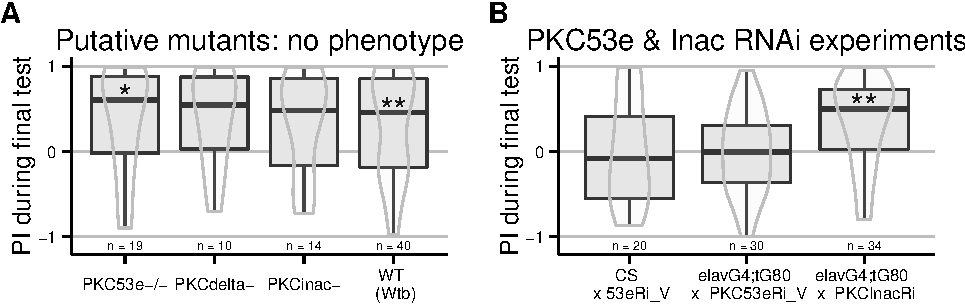
\includegraphics{firsttest_files/figure-latex/unnamed-chunk-2-1.pdf}
\caption{\label{fig:PKC} Failed attempts to identify the PKC gene
involved in operant self-learning. Performance indexes (PI) during a
test period following an 8 min. training session is reported. LEFT:
Flies putatively mutants for PKC genes (PKC-53e, PKC-delta and PCK-InaC)
performed well in the self-learning assay. RIGHT: Flies with RNAi
constructs targeting PKC53e and PKC InaC were crossed to
elav-Gal4;tub-Gal80ts or to CS females. RNAi was induced for two days
before the experiment via a 32 degrees heat-shock. While the construct
targeting PKC InaC had no effect, the construct for PKC53e prevented
self-learning formation even in absence of Gal4 driven expression, such
that no firm conclusions can be drawn. Full genotype of the flies tested
is indicated below. CS x 53eRi\_V : ;;UAS\_PKC53eRNAi\_27696/+ .
elavG4;tG80 x PKC53eRi\_V :
elavGal4/+;tubGal80ts/+;UAS\_PKC53eRNAI\_27696/+ . elavG4;tG80 x
PKCInacRi : elavGal4/+;tubGal80ts/+;UAS\_PKCInacRNAI\_2895/+. Data is
shown as Tukey's boxplots (median is the line surrounded by boxes
representing quartiles) with a superposed violinplot. Asterisks indicate
significant difference of the score against 0, using a non-parametrical
Wilcox test.}
\end{figure}

\begin{figure}[htbp]
\centering
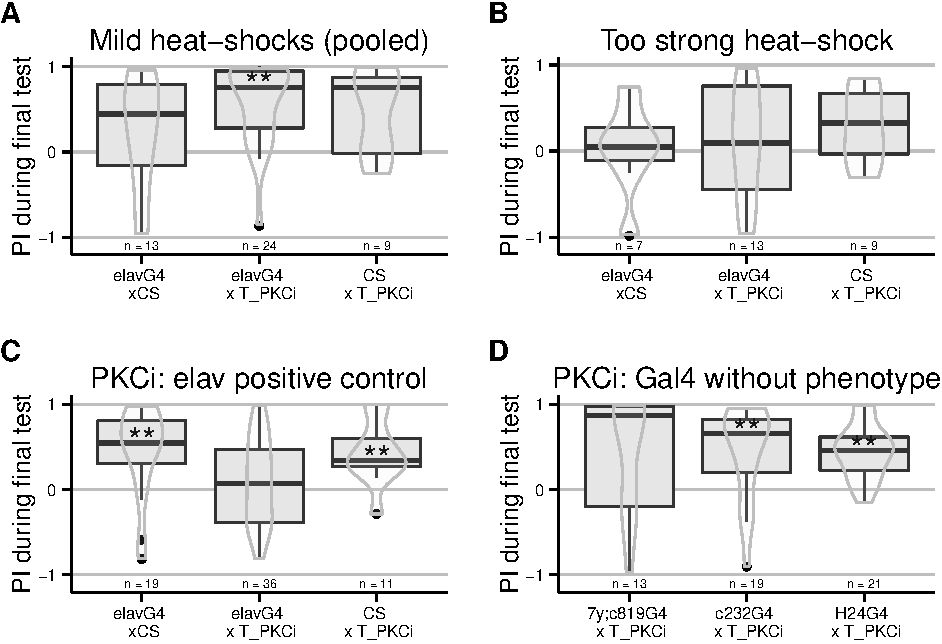
\includegraphics{firsttest_files/figure-latex/unnamed-chunk-3-1.pdf}
\caption{\label{fig:heatshock} PKC inhibition (achieved by using an
effective heat-shock protocol) in neurons, but not central brain
regions, prevents self-learning formation. Driving Gal4 in all neurons
using the elav-Gal4 driver while inactivating its ubiquitously expressed
inhibitor Gal80 with a heat-shock induces the expression of the PKC
inhibitor. While test flies are still performing well after a mild
heat-shock (A, data pooled from different protocols: 33° for 15h, 36°
for 2h, and 37°for 1h), a strong heat-shock prevents learning in control
flies (B, 37° for 2h). After a 4-hour heat-shock at 35°C, test but not
control flies were unable to form self-learning (C). Using this latter
protocol, we restricted the expression of Gal4 in central brain regions
using different drivers targeting central brain regions (D), which were
all ineffective in preventing self-learning. Full genotype of the flies
tested is indicated below. elavG4 xCS : elav-Gal4/+ . elavG4 x T\_PKCi :
elav-Gal4/+;tubGal80ts/+ ; UAS-PKCi/+ . CS x T\_PKCi : tubGal80ts/+ ;
UAS-PKCi/+. 7y;c819G4 x T\_PKCi : tubGal80ts/+ ; UAS-PKCi/+ \_\_
H24-Gal4 . c232G4 x T\_PKCi : tubGal80ts/+ ; UAS-PKCi/7y\_Gal4,c819-Gal4
. H24G4 x T\_PKCi : tubGal80ts/+ ; UAS-PKCi/c232-Gal4. Data is shown as
Tukey's boxplots (median is the line surrounded by boxes representing
quartiles) with a superposed violinplot. Asterisks indicate significant
difference of the score against 0, using a non-parametrical Wilcox
test.}
\end{figure}

\begin{figure}[htbp]
\centering
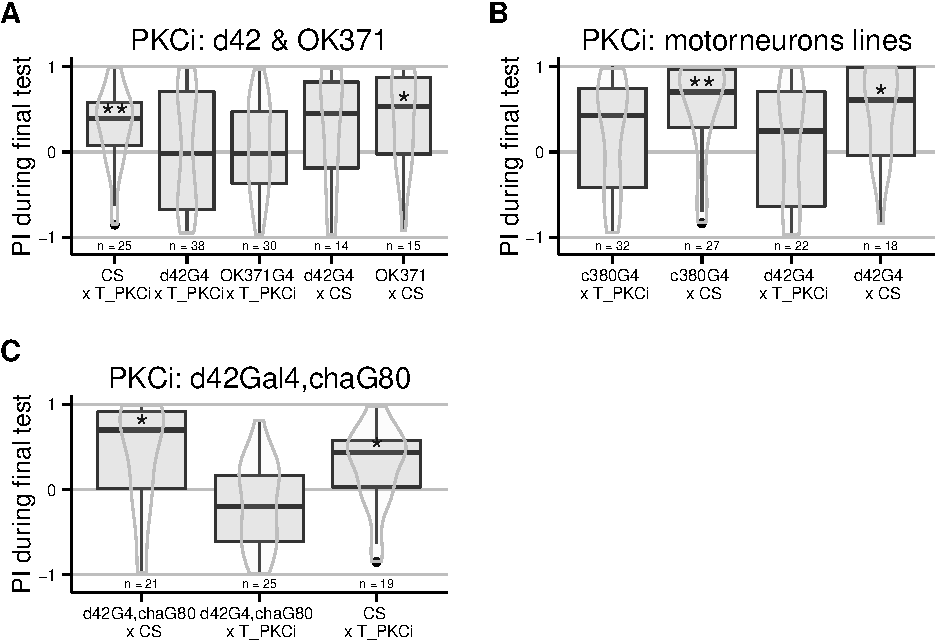
\includegraphics{firsttest_files/figure-latex/unnamed-chunk-4-1.pdf}
\caption{\label{fig:motoneurons} Flies with PKCi expression in
motorneurons, are impaired in self-learning. A. Using OK371-Gal4
(expression in most glutamatergic neurons) or d42-Gal4 to drive PKCi
expression was effective in preventing self-learning, while the control
flies seem to learn, although the score of the d42Gal4 x CS control line
was not statistically significantly positive. B. While the previous
result with the D42Gal4 driver was reproduced, using c380-Gal4, a second
driver showing expression in motorneurons, yielded comparable results.
C. The use of the d42Gal4,chaGal80 double construct as a driver was
effective in preventing self-learning, while the controls did perform
well. Heat-shock protocol was a 4-hour heat-shock at 35°C. Full genotype
of the flies tested is indicated below. CS x T\_PKCi : tubGal80ts/+ ;
UAS-PKCi/+ . d42G4 x T\_PKCi : tubGal80ts/+ ; UAS-PKCi/d42-Gal4 .
OK371G4 x T\_PKCi : tubGal80ts/+ ; UAS-PKCi/+;OK371/+ . d42G4 x CS :
d42Gal4/+ . OK371 x CS : OK371/+ .c380G4 x T\_PKCi : c380-Gal4/+ .
c380G4 x CS : c380Gal4/+; tubGal80ts/+ ; UAS-PKCi/+ . d42G4,chaG80 x CS
: d42-Gal4, cha-Gal80/+ . d42G4,chaG80 x T\_PKCi : tubGal80ts/+ ;
UAS-PKCi/d42-Gal4, cha-Gal80 . CS x T\_PKCi : tubGal80ts/+ ; UAS-PKCi/+.
Data is shown as Tukey's boxplots (median is the line surrounded by
boxes representing quartiles) with a superposed violinplot. Asterisks
indicate significant difference of the score against 0, using a
non-parametrical Wilcox test.}
\end{figure}

\end{document}
